\documentclass[letterpaper,12pt]{article}
\usepackage[letterpaper, portrait, margin=0.5in]{geometry}
\usepackage{graphicx}
\usepackage{multicol}
\graphicspath{{images/}}
\newcommand\numbox{%%
    \fbox{\rule{1in}{0pt}\rule[-1ex]{0pt}{5ex}}}
\usepackage[utf8]{inputenc}
\usepackage[english]{babel}
\usepackage{multicol}
\graphicspath{{images/}}
\usepackage[export]{adjustbox}

\begin{document}
\noindent No escriba su nombre debajo de esta línea. \\
\noindent \hrule
\begin{center}
{\Large \textbf{\underline{Bucles}}} \\
\end{center}
Nombre de usuario de Scratch: \rule{4cm}{0.4pt}

\noindent \dotfill


\begin{center}
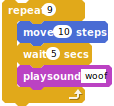
\includegraphics[scale=.6]{q1_script0.png}
\end{center}
1. Cuántas veces repiten los bloques en el bucle?
\numbox \\

\noindent \dotfill
\begin{center}
\includegraphics[scale=.7]{q2_script0.png}
\end{center}

\noindent 2. \textbf{Circula} el script que hace que el sprite haga lo mismo que en el bucle anteriormente.: \\ \\
\includegraphics[scale=.6,valign=t]{q2_script1.png} \hspace{1.25cm}
\includegraphics[scale=.6,valign=t]{q2_script2.png} \hspace{1.25cm}
\includegraphics[scale=.6,valign=t]{q2_script3.png} \hspace{1.25cm}
\includegraphics[scale=.6,valign=t]{q2_script4.png} \hspace{1.25cm}

\noindent \dotfill

\noindent 3. \textbf{Circula \underline{TODOS}} los scripts que hace que el sprite cambie su disfraz 3 veces.  \\

\includegraphics[scale=.6,valign=t]{q3_script0.png} \hspace{1.5cm}
\includegraphics[scale=.6,valign=t]{q3_script1.png} \hspace{1.5cm}
\includegraphics[scale=.6,valign=t]{q3_script2.png} \hspace{1.5cm}
\includegraphics[scale=.6,valign=t]{q3_script3.png} \hspace{1.5cm} \\


\noindent \dotfill

\begin{center}
\includegraphics[scale=.7]{q4_script0.png}
\end{center}

\noindent 4. \textbf{Circula} el script que hace que el sprite haga lo mismo que en el bucle anteriormente.: \\ \\
\includegraphics[scale=.625,valign=t]{q4_script1.png} \hspace{.01cm}
\includegraphics[scale=.625,valign=t]{q4_script2.png} \hspace{.01cm}
\includegraphics[scale=.625,valign=t]{q4_script3.png} \hspace{.01cm}
\includegraphics[scale=.625,valign=t]{q4_script4.png} \hspace{.01cm}

\noindent \dotfill

\begin{center}
\includegraphics[scale=.75]{q5_script0.png}
\end{center}

\noindent 5a. \textbf{Circula \underline{TODOS}} los bloques que corren 6 veces en el script anteriormente. \\ \\
\includegraphics[scale=.8]{q5_script1.png} \hspace{1cm}
\includegraphics[scale=.8]{q5_script2.png} \hspace{1cm}
\includegraphics[scale=.8]{q5_script3.png} \hspace{1cm}
\includegraphics[scale=.8]{q5_script4.png} \hspace{1cm}\\

\noindent 5b. \textbf{Circula \underline{TODOS}} los bloques que corren \underline{antes} que el bucle anteriormente.  \\ \\
\includegraphics[scale=.8]{q5_script1.png} \hspace{1cm}
\includegraphics[scale=.8]{q5_script2.png} \hspace{1cm}
\includegraphics[scale=.8]{q5_script3.png} \hspace{1cm}
\includegraphics[scale=.8]{q5_script4.png} \hspace{1cm}\\

\noindent 5c. \textbf{Circula \underline{TODOS}} los bloques que corren \underline{después} de el bucle anteriormente.  \\ \\
\includegraphics[scale=.8]{q5_script1.png} \hspace{1cm}
\includegraphics[scale=.8]{q5_script2.png} \hspace{1cm}
\includegraphics[scale=.8]{q5_script3.png} \hspace{1cm}
\includegraphics[scale=.8]{q5_script4.png} \hspace{1cm}\\

\noindent \dotfill \\

\newpage

\indent \includegraphics[scale=.25,valign=c]{cat.png} \underline{Código de el Gato} \hspace{5cm}
\includegraphics[scale=.2,valign=c]{dog.png} \underline{Código de el Perro} \\
\includegraphics[scale=.8,valign=t]{q6_script0.png} \hspace{1cm}
 \vline height .75cm width 2pt \hspace{1cm}
\includegraphics[scale=.8, valign=t]{q6_script1.png} \hspace{1cm}
\includegraphics[scale=.8, valign=t]{q6_script2.png} \\ 

\noindent 6a. \textbf{Circula}: ¿Cuando se hace clic en la bandera verde, que va hacer el gato?
\renewcommand{\theenumi}{\Alph{enumi}}
\begin{enumerate}
\item El gato dice “meow” 7 veces y el disfraz se cambia 4 veces. 
\item El gato dice “meow” y cambia su disfraz \textbf{al mismo tiempo}. \\
\end{enumerate}

\noindent 6b. \textbf{Circula}: ¿Cuándo se hace clic en la bandera verde, que hace el perro?
\renewcommand{\theenumi}{\Alph{enumi}}
\begin{enumerate}
\item El perro dice “woof” 7 veces y el disfraz se cambia 4 veces.
\item El perro dice “woof” y cambia su disfraz \textbf{al mismo tiempo}.
\end{enumerate}

\noindent \dotfill

\begin{center}
\includegraphics[scale=.8]{q7_script0.png}
\end{center}
7. Explica lo que este script hará que el sprite haga. \\
Cada ves que el bucle corre: \\ \\
\indent Primero, \hrulefill. \\ \\
\indent Siguiente, \hrulefill. \\ \\
\indent Ultimo, \hrulefill. \\ \\
 Esto pasa \rule{1cm}{0.5pt} veces. \\

\noindent ¡Mas preguntas en la próxima pagina! \dotfill \\

\noindent 8. Como sabe que debes de usar un bucle?  \\ \\
\noindent \rule{18.5cm}{0.5pt} \\ \\
\noindent \rule{18.5cm}{0.5pt} \\ \\
\noindent \rule{18.5cm}{0.5pt} \\

\noindent \dotfill \\
\begin{center}
\includegraphics[scale=.8]{ec_script0.png}
\end{center}

\noindent \textbf{Extra Challenge:}¿Cuantas veces se reproduce el sonido “quack”? \numbox
\end{document}